\section{Recorded Retrieval Results}\label{sec:results}
\subsection{Effectiveness under the declared configurations}
Table~\ref{tab:headline} reports the selected full-test policies. The values come from the completed studies; no new journal experiments were collected. The reported nDCG@5 values are \scifactNdcg{}, \nfcorpusNdcg{}, and \fiqaNdcg{} on SciFact, NFCorpus, and FiQA, respectively. In the first two rows, nDCG@5 is tied to the matched base by prefix preservation. FiQA's row instead reports the earlier fifteen-candidate base selector. The configuration label is therefore necessary to interpret the result.

\begin{table}[t]
\centering\small\setlength{\tabcolsep}{3pt}
\caption{Reported full-test policies. SciFact/NFCorpus include refinement; FiQA uses the earlier base. All quantities within a row come from the same recorded policy.}
\label{tab:headline}\begin{tabular}{lrrrr}
\toprule
Dataset & nDCG@5 & nDCG@8 & Recall@8 & Redundancy $\downarrow$\\
\midrule
SciFact & 0.687833 & 0.698173 & 0.801111 & 0.433636\\
NFCorpus & 0.368865 & 0.346506 & 0.152997 & 0.431771\\
FiQA & 0.357490 & 0.376939 & 0.434063 & 0.531244\\
\bottomrule
\end{tabular}

\end{table}

Relative to matched base selection, SciFact refinement reduces mean redundancy by \scifactRedReduction\% and changes mean Recall@8 by \scifactRecallChange\% relative. NFCorpus reduces redundancy by \nfcorpusRedReduction\% with a +\nfcorpusRecallChange\% relative recall change. The recall changes have different signs across domains. The refinement therefore cannot be described as a general recall improvement, even though the same prefix metric is preserved on both collections.

The FiQA base reaches Recall@8 of \fiqaRecall{} and redundancy of \fiqaRedundancy{}. It matches the reported nDCG@5 and recall of its same-shortlist L6-only control. A later, separately completed 648-query FiQA refinement follow-up preserved nDCG@5 and reduced redundancy by \fiqaFollowupRedReduction\%, but lost \fiqaFollowupRecallLoss\% relative recall. That result failed the frozen 98\% recall-retention gate and was not retuned into a passing result. We retain the prior manuscript's disclosure of this failure without substituting its redundancy value into the earlier base row.

\subsection{Classical and neural comparisons}
Table~\ref{tab:comparators} places the reported policy alongside the declared controls. The cross-encoder shortlist distinctions matter: L6-only uses hybrid fifteen, while the dense-fifteen neural control uses the fifteen highest dense-scoring parents. Differences between those rows include candidate construction. Dense-sixty-four neural reranking additionally exposes the relevance model to more candidates and incurs the corresponding inference cost.

\begin{table*}[t]
\centering\small\setlength{\tabcolsep}{4pt}
\caption{Recorded full-test comparison. n@5 is nDCG@5, R@8 is Recall@8, and Red. is redundancy. Matched search controls use the refined domain on SciFact/NFCorpus and the base domain on FiQA. Additional saved methods remain in the complete CSV export.}
\label{tab:comparators}\begin{tabular}{lrrrrrrrrr}
\toprule
& \multicolumn{3}{c}{SciFact} & \multicolumn{3}{c}{NFCorpus} & \multicolumn{3}{c}{FiQA}\\
Policy & n@5 & R@8 & Red. & n@5 & R@8 & Red. & n@5 & R@8 & Red.\\
\midrule
Dense cosine & 0.6361 & 0.8111 & 0.4756 & 0.3181 & 0.1335 & 0.4398 & 0.3470 & 0.4153 & 0.5363\\
Dense/BM25 RRF & 0.6677 & 0.8149 & 0.4727 & 0.3491 & 0.1394 & 0.4394 & 0.3509 & 0.4262 & 0.5327\\
Legacy threshold Grover & 0.6364 & 0.8111 & 0.4756 & 0.3181 & 0.1334 & 0.4398 & 0.3458 & 0.4150 & 0.5363\\
Cosine-guided GAS & 0.6311 & 0.7742 & 0.4490 & 0.3160 & 0.1235 & 0.3996 & 0.3452 & 0.4093 & 0.5215\\
L6 relevance only & 0.6878 & 0.8086 & 0.4480 & 0.3689 & 0.1500 & 0.4447 & 0.3575 & 0.4341 & 0.5313\\
L6 MMR & 0.6878 & 0.8086 & 0.4480 & 0.3689 & 0.1500 & 0.4447 & 0.3575 & 0.4341 & 0.5313\\
Base L6-guided GAS & 0.6878 & 0.8086 & 0.4480 & 0.3689 & 0.1501 & 0.4434 & 0.3575 & 0.4341 & 0.5312\\
Matched greedy & 0.6878 & 0.8011 & 0.4336 & 0.3689 & 0.1530 & 0.4318 & 0.3575 & 0.4341 & 0.5311\\
Matched exact float & 0.6878 & 0.8011 & 0.4336 & 0.3689 & 0.1530 & 0.4318 & 0.3575 & 0.4343 & 0.5309\\
Matched exact integer & 0.6878 & 0.8011 & 0.4336 & 0.3689 & 0.1530 & 0.4318 & 0.3575 & 0.4341 & 0.5311\\
Matched random & 0.6878 & 0.8011 & 0.4338 & 0.3689 & 0.1531 & 0.4320 & 0.3575 & 0.4341 & 0.5313\\
L2, dense 15 & 0.6431 & 0.8049 & 0.4642 & 0.3509 & 0.1396 & 0.4486 & 0.3319 & 0.4217 & 0.5295\\
L6, dense 15 & 0.6790 & 0.8104 & 0.4655 & 0.3621 & 0.1423 & 0.4537 & 0.3575 & 0.4341 & 0.5313\\
L2, dense 64 & 0.6321 & 0.7916 & 0.4329 & 0.3481 & 0.1438 & 0.4468 & 0.2973 & 0.3918 & 0.4962\\
L6, dense 64 & 0.6815 & 0.8087 & 0.4379 & 0.3670 & 0.1437 & 0.4586 & 0.3535 & 0.4160 & 0.5033\\
Reported GAS policy & 0.6878 & 0.8011 & 0.4336 & 0.3689 & 0.1530 & 0.4318 & 0.3575 & 0.4341 & 0.5312\\
\bottomrule
\end{tabular}

\end{table*}

Matched greedy and exact-float refiners have the same aggregate nDCG@5, nDCG@8, Recall@8, and redundancy as constrained GAS on the SciFact and NFCorpus tests. This agreement shows that the measured quality of those outputs does not depend on the Grover search mechanism. The constrained objective and the available candidates explain a benefit that several optimizers can realize.

Table~\ref{tab:expanded} further separates candidate expansion, prefix retention, and constrained set optimization. Global union-L6 permits complete reordering. Protected-prefix union-L6 preserves the head but chooses the tail by neural relevance. The constrained optimizers additionally optimize pair redundancy under the score thresholds. These controls address different sources of change; grouping them under one generic ``reranking'' label would obscure the mechanism being evaluated.

\begin{table*}[t]
\centering\small\setlength{\tabcolsep}{4pt}
\caption{Expanded-pool controls on the two protected-refinement test runs. All four metrics are shown to expose tail effects hidden by a fixed top five. FiQA has no corresponding expanded-pool headline in the selected source mapping.}
\label{tab:expanded}\begin{tabular}{lrrrrrrrr}
\toprule
& \multicolumn{4}{c}{SciFact} & \multicolumn{4}{c}{NFCorpus}\\
Policy & n@5 & n@8 & R@8 & Red. & n@5 & n@8 & R@8 & Red.\\
\midrule
Union L6, global order & 0.6860 & 0.6972 & 0.8037 & 0.4475 & 0.3688 & 0.3472 & 0.1522 & 0.4477\\
Union L6, protected prefix & 0.6878 & 0.6993 & 0.8037 & 0.4474 & 0.3689 & 0.3466 & 0.1523 & 0.4474\\
Constrained GAS & 0.6878 & 0.6982 & 0.8011 & 0.4336 & 0.3689 & 0.3465 & 0.1530 & 0.4318\\
Constrained greedy & 0.6878 & 0.6982 & 0.8011 & 0.4336 & 0.3689 & 0.3465 & 0.1530 & 0.4318\\
Constrained exact float & 0.6878 & 0.6982 & 0.8011 & 0.4336 & 0.3689 & 0.3465 & 0.1530 & 0.4318\\
Constrained exact integer & 0.6878 & 0.6982 & 0.8011 & 0.4336 & 0.3689 & 0.3465 & 0.1530 & 0.4318\\
Constrained random & 0.6878 & 0.6982 & 0.8011 & 0.4338 & 0.3689 & 0.3468 & 0.1531 & 0.4320\\
\bottomrule
\end{tabular}

\end{table*}

The observed tradeoffs are visualized in Fig.~\ref{fig:tradeoffs}. Some inexpensive or less relevance-focused policies have lower redundancy while also having lower recall. The graph contains measured operating points, not a tuned Pareto frontier or a proof of dominance over every possible setting. In particular, the zero-diversity MMR point does not represent the complete range of MMR operating choices.

\begin{figure*}[t]
\centering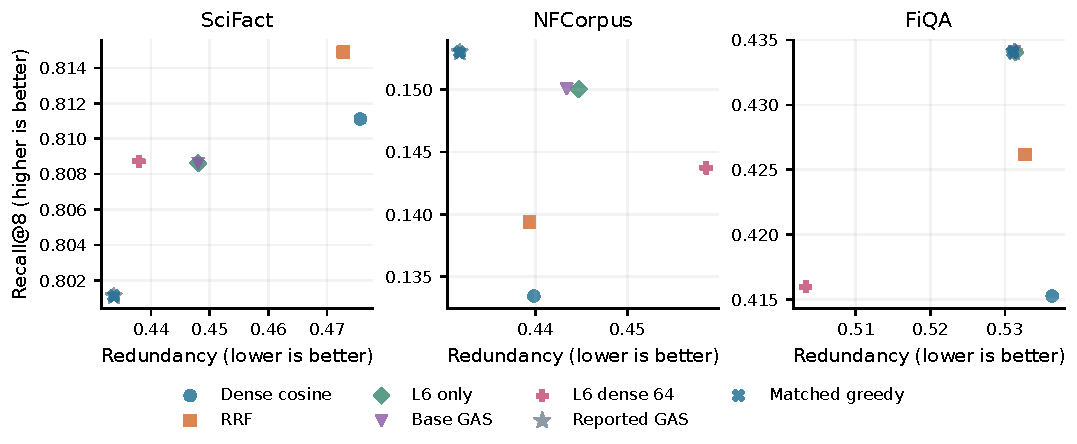
\includegraphics[width=\textwidth]{observed_tradeoffs.pdf}
\caption{Observed Recall@8--redundancy operating points from the saved runs. Coincident points can arise when policies return the same effective outputs. Candidate pools differ as specified in the protocol; the graph is descriptive and does not imply matched causal comparisons across every point.}
\label{fig:tradeoffs}
\end{figure*}

\subsection{Paired uncertainty and interpretation}
Table~\ref{tab:statistics} reproduces paired differences against the base for the protected datasets. SciFact's recall interval includes both a loss and a gain, while its mean is negative. NFCorpus's positive recall interval is pointwise; the recorded raw probability does not produce a rejection after the complete Holm family is considered. The distinction between a displayed interval and a familywise testing decision must remain explicit.

\begin{table*}[t]
\centering\small
\caption{Recorded paired inference: reported refinement minus base on SciFact/NFCorpus. $\dagger$FiQA is its earlier base minus L6-only for the independently audited nDCG@5 comparison. Intervals are pointwise, not simultaneous; Holm decisions use each original full family.}
\label{tab:statistics}\begin{tabular}{llrrrc}
\toprule
Dataset & Metric & Mean difference & Paired 95\% CI & Raw $p$ & Holm reject\\
\midrule
SciFact & nDCG@5 & +0.00000 & [+0.00000, +0.00000] & 1.00000 & No\\
SciFact & nDCG@8 & -0.00268 & [-0.00811, +0.00231] & 0.30427 & No\\
SciFact & Recall@8 & -0.00750 & [-0.02417, +0.00750] & 0.45645 & No\\
SciFact & Redundancy & -0.01439 & [-0.01680, -0.01216] & 0.00010 & Yes\\
NFCorpus & nDCG@5 & +0.00000 & [+0.00000, +0.00000] & 1.00000 & No\\
NFCorpus & nDCG@8 & +0.00094 & [-0.00248, +0.00445] & 0.58974 & No\\
NFCorpus & Recall@8 & +0.00293 & [+0.00038, +0.00622] & 0.03690 & No\\
NFCorpus & Redundancy & -0.01165 & [-0.01405, -0.00938] & 0.00010 & Yes\\
FiQA & nDCG@5$^\dagger$ & 0.00000 & [0.00000, 0.00000] & 1.00000 & No\\
\bottomrule
\end{tabular}

\end{table*}

The empirical 98\% mean-recall gate is not a statistical noninferiority test, and an interval containing zero does not establish equivalence. Stronger inferential claims would require a justified noninferiority margin, a prospective analysis, and data whose role in method development is appropriately controlled. The present evidence supports the recorded descriptive gate outcomes and the stated paired comparisons.

The FiQA statistical audit also illustrates why floating-point conventions matter. Averaging five identical seeded scores can produce a difference of approximately one unit in the last place relative to a deterministic control. A significance test must not promote that numerical artifact into evidence of a retrieval improvement. The recorded $10^{-12}$ tie policy addresses this problem while leaving rankings and reported raw means intact.

\subsection{Latency and optimization outcomes}
Complete online median and P95 times appear in Table~\ref{tab:latency}. Expanded-pool inference increases complete latency relative to the matched base. A small refinement time does not make the two-stage pipeline equally inexpensive. Comparisons with dense-sixty-four rerankers involve both cost and candidate opportunity and should not be reduced to a universal speed claim.

\begin{table*}[t]
\centering\small\setlength{\tabcolsep}{6pt}
\caption{Composed online latency, milliseconds per seeded request. Values include all applicable upstream stages. P50/P95 are computed over recorded request totals; restoration, model loading, and warm-up are separate.}
\label{tab:latency}\begin{tabular}{lrrrrrr}
\toprule
& \multicolumn{2}{c}{SciFact} & \multicolumn{2}{c}{NFCorpus} & \multicolumn{2}{c}{FiQA}\\
Policy & P50 & P95 & P50 & P95 & P50 & P95\\
\midrule
Dense cosine & 33.3 & 48.3 & 24.5 & 32.9 & 79.9 & 98.5\\
Dense/BM25 RRF & 61.6 & 94.9 & 31.0 & 44.5 & 225.3 & 328.3\\
Legacy threshold Grover & 38.2 & 313.6 & 25.2 & 281.6 & 84.3 & 231.9\\
Cosine-guided GAS & 42.3 & 56.8 & 33.7 & 42.0 & 84.1 & 102.5\\
L6 relevance only & 955.3 & 1085.4 & 851.9 & 901.4 & 650.0 & 821.1\\
L6 MMR & 955.5 & 1085.7 & 852.1 & 901.6 & 650.1 & 821.3\\
Base L6-guided GAS & 963.2 & 1093.7 & 859.8 & 909.1 & 653.8 & 826.7\\
Matched greedy & 1405.4 & 1670.7 & 1145.5 & 1479.6 & 650.0 & 821.2\\
Matched exact float & 1405.2 & 1670.6 & 1145.3 & 1479.3 & 651.2 & 822.5\\
Matched exact integer & 1405.2 & 1670.6 & 1145.3 & 1479.3 & 651.1 & 822.4\\
Matched random & 1405.2 & 1670.6 & 1145.4 & 1479.3 & 651.9 & 824.8\\
L2, dense 15 & 348.0 & 403.0 & 310.5 & 331.5 & 238.9 & 294.6\\
L6, dense 15 & 915.8 & 1029.2 & 832.5 & 882.5 & 539.6 & 618.2\\
L2, dense 64 & 1374.7 & 1562.5 & 1242.5 & 1319.6 & 763.7 & 912.2\\
L6, dense 64 & 3799.0 & 4322.2 & 3460.8 & 3630.9 & 2037.9 & 2437.9\\
Reported GAS policy & 1406.5 & 1672.3 & 1146.8 & 1481.3 & 653.8 & 826.7\\
\bottomrule
\end{tabular}

\end{table*}

Table~\ref{tab:search} distinguishes logical work from outcome quality. An exact objective hit is evaluated against the corresponding exact float-redundancy optimum for refinement and the exact integer optimum for the base. Such a hit certifies neither maximum judged recall nor maximum nDCG. Budget exhaustion, a trivial basis, and an unchanged incumbent are meaningful outcomes retained in the request denominator.

\begin{table*}[t]
\centering\small
\caption{Recorded search work and combined selector latency in milliseconds. The first phase column counts inherited base work for refined policies; it is zero for base-only FiQA. The next column counts the current stage. Optimum-hit definitions follow the text.}
\label{tab:search}\begin{tabular}{lrrrrrr}
\toprule
Dataset & Requests & Base phases & Refine/base phases & Optimum-hit rate & Selector P50 & Selector P95\\
\midrule
SciFact & 1500 & 64.00 & 20.08 & 1.000 & 9.66 & 10.67\\
NFCorpus & 1615 & 63.91 & 17.82 & 1.000 & 9.49 & 11.02\\
FiQA & 3240 & 0.00 & 64.00 & 0.994 & 3.95 & 4.54\\
\bottomrule
\end{tabular}

\end{table*}

The work counts document this implementation's behavior. They cannot establish physical acceleration: the CPU simulator prepares the complete objective array, and classical methods can inspect that array directly. The objective assumptions and measured cost boundaries remain explicit.
